\documentclass[a4paper,10pt]{article}
\usepackage[utf8]{inputenc}
 
% Blank line between paragraphs instead of indenting the first line
\usepackage{parskip}
\setlength{\parskip}{\baselineskip}

% Squash a bit more text onto a page
\usepackage{geometry}
\geometry{verbose,tmargin=20mm,bmargin=20mm,lmargin=20mm,rmargin=20mm}

\usepackage{graphicx}
\usepackage{listings}
\usepackage{amsmath}
\usepackage{verbatim}
\usepackage{color}
\usepackage{wrapfig}
\usepackage{subcaption}

% Indent verbatim environments
\makeatletter \def\verbatim@processline{\hspace*{2em}\the\verbatim@line\par}\makeatother

\definecolor{mygreen}{rgb}{0,0.6,0}
\definecolor{mygray}{rgb}{0.5,0.5,0.5}
\definecolor{mymauve}{rgb}{0.58,0,0.82}

\lstset { 
  backgroundcolor=\color{white},   % choose the background color; you must add \usepackage{color} or \usepackage{xcolor}
  basicstyle=\footnotesize,        % the size of the fonts that are used for the code
  breakatwhitespace=false,         % sets if automatic breaks should only happen at whitespace
  breaklines=true,                 % sets automatic line breaking
  captionpos=b,                    % sets the caption-position to bottom
  commentstyle=\color{mygreen},    % comment style
  deletekeywords={...},            % if you want to delete keywords from the given language
  escapeinside={\%*}{*)},          % if you want to add LaTeX within your code
  extendedchars=true,              % lets you use non-ASCII characters; for 8-bits encodings only, does not work with UTF-8
  frame=single,                    % adds a frame around the code
  keepspaces=true,                 % keeps spaces in text, useful for keeping indentation of code (possibly needs columns=flexible)
  keywordstyle=\color{blue},       % keyword style
  language=C++,                    % the language of the code
  morekeywords={*,DEVICES,
  				CONNECTIONS,
  				MONITORS,
  				END}, 	           % if you want to add more keywords to the set
  numbers=left,                    % where to put the line-numbers; possible values are (none, left, right)
  numbersep=5pt,                   % how far the line-numbers are from the code
  numberstyle=\tiny\color{mygray}, % the style that is used for the line-numbers
  rulecolor=\color{black},         % if not set, the frame-color may be changed on line-breaks within not-black text (e.g. comments (green here))
  showspaces=false,                % show spaces everywhere adding particular underscores; it overrides 'showstringspaces'
  showstringspaces=false,          % underline spaces within strings only
  showtabs=false,                  % show tabs within strings adding particular underscores
  stepnumber=1,                    % the step between two line-numbers. If it's 1, each line will be numbered
  stringstyle=\color{mymauve},     % string literal style
  tabsize=2,                       % sets default tabsize to 2 spaces
  title=\lstname                   % show the filename of files included with \lstinputlisting; also try caption instead of title
}

\begin{document}
%\contentsname{IIA GF2 Software: Final Report}
\begin{center}
\Huge \textbf{IIA GF2 Software: Final Report}

\large Tim Hillel (th389) \\ Team 8 \\ Downing College
\end{center}

\tableofcontents
\pagebreak

\section{Description}
The aim of the project was to implement a logic simulator that is able to simulate logic circuits which include the following devices:

\begin{itemize}
\item Clocks
\item Switches
\item AND gates (Up to 16 inputs)
\item NAND gates (Up to 16 inputs)
\item OR gates (Up to 16 inputs)
\item NOR gates (Up to 16 inputs)
\item XOR gates
\item D-Type flip-flops
\item Signal generators


\begin{figure}[h]
 \centering
 %\includegraphics[width=8cm]{../docs/uml.png}
 \caption{UML Class diagram of our logic simulator}
 \label{fig:uml}
\end{figure}


\end{itemize}
\pagebreak
\section{Teamwork and Development Style}

In the project planning stage, we split the development of our logic simulator into five major phases: specification, design, implementation, testing and maintenance. The timeframe was then decided for each task and each task was assigned to either a team member or the whole team, depending on the nature of the task. This is shown in the Gantt chart in Appendix F. Overall we found we stuck well to the planned timescale, often completing tasks before the internal deadlines we had set, which allowed longer for incremental improvements to code in the testing and debugging stages.

Each member of the team was also assigned a general project role as follows:

\textbf{Project manager:} (T Hillel) - Responsible for project planning including delegation of tasks and ensuring that the project runs to the set timescale.

\textbf{Programming administrator:} (J Magee) - Responsible for upkeep of the project directory including performing builds and keeping legacy versions of the simulator.

\textbf{Client representative:} (M Jackson) - Responsible for ensuring that the project meets the client's requirements for the logic simulator as defined in Appendix A of the GF2 Project Handout.

Overall this system worked relatively effectively, as each member of the team had both technical and general tasks which they were responsible for. We did find during the running of the project that there was not a strong need for a strict organisational structure. This was mainly due to the extensive use of git for revision control through GitHub. This allowed each member of the team to test, edit and change any code within the project remotely, whilst fully tracking any changes made to code. GitHub allowed issues to be raised when bugs were found that would require more than a quick fix or when functionality of a class did not exactly meet the client's specification.

Occassionally this allowed for problems when multiple users edited the same file before attempting to push it to the repository, but \texttt{git merge} was used to deal with these issues effectively.

We also found that the breakdown of the tasks we had initially planned for were not completely equal, as an example the names and scanner class implemented a lot of the code written in the preliminary exercises, and so Jamie Magee, who was assigned to this task, had time to help me with the parser. GitHub allowed the team to track which tasks required more input and so a member could assist when they had finished their section, such as Jamie Magee helping with \texttt{parser.cc}. Whilst Martin Jackson's primary task was the GUI during the developement phase, he was also always on hand to help debug problems in the other classes.

For the maintenance phase of the project, each team member was assigned to one of the modifications required:

\textbf{Nonzero Hold Time of Bistables:} J Maggee

\textbf{Signal Generators:} T Hillel

\textbf{Continious Simulation:} M Jackson

Again we found that the tasks were not balanced; the nonzero hold time of bistables modification was a more involved task, and so Martin Jackson helped Jamie Maggee with this task whilst I implemented general maintenance changes as suggested by feedback from Interim Report 2.

Overall, the team worked very effectively through the task and there were no issues that caused any major problems. Using GitHub to manage the task definitely aided with the efficeincy of the team, and the experience has provided useful skills for the future.

\section{My Contribution}

For the design and implementation stages of the project, I was mainly responsible for the parser and error detection, which was implemented in a seperate error class. The parser operates by calling the scanner class, which has internal functions to skip whitspace and comments, returning the code one symbol at a time, out of \texttt{namesym, numsym, devsym, consym, monsym, endsym, classsym, iosym, colon, semicol, equals, dot, badsym} and \texttt{eofsym}. If the symbol is not the one expected according to the EBNF, an error function is called in the error class, passing the associated error code. The error class then looks up the error code on a lookup table, which is a vector of error messages, and outputs the error message, as well as increasing the \textt{errorCount}. A function is also called in the scanner class, which outputs the line the error occured on as well as where on the line the error occured, up to the next semicolon. Parsing then continues from the next line.

Warnings were implemented using a similar technique, except warnings within the error class do not call the function outputting the line and position the error occured on, as this would cause code to be skipped by the parser. Instead, where a warning needed to output more specific information, for instance the specific output that was being monitered multiple times, this information was parsed from the parser to the warning function within the errors class, and outputted along with the warning message.

To help with the readability of the code, each line of the EBNF was implemented as a seperate function within the parser.

Within the maintenance phase, I was responsible for implementing signal generators within the logic simulator. This involved modifying all of the scanner, names, parser, devices and error classes, as well as the EBNF. Changes within the GUI were handled by Martin Jackson. The majority 

\section{Testing}

We used two main tests of testing - unit and system testing - both of which are industry standard practices. For our unit testing, Martin wrote an errors class which compared the actual output from various units of code, to the expected output. For system testing I wrote a shell script which passed definition files to the logic simulator and recorded the output in a text file. There were two variatons on the shell script: One which ran known good definition files and therefore had to input the commands to run the simulation in addition to recording the output; Another which ran known bad definition files and only expected parsing errors which it recorded.

\section{Conclusions}

\pagebreak

\appendix
\section{Code Listings}
Please see attatched Interim Report 2 for all code listings.

\section{Test Definition Files}

Shown below are the test definition files for funcionality added in the maintenance phase of the project.

Please see attatched Interim Report 2 for test definition files for functions implemented up to section 10 of the project.

\subsection{SIGGEN}

\subsubsection{Definition File}
\lstinputlisting[caption=siggen.gf2 - Note defined a very long waveform to test ability to take waveform of arbritary length; defined other waveform with spaces in sequence to test this ability]{../../examples/siggen.gf2}

\subsubsection{Circuit Diagram}
\begin{figure}[h]
 \centering
 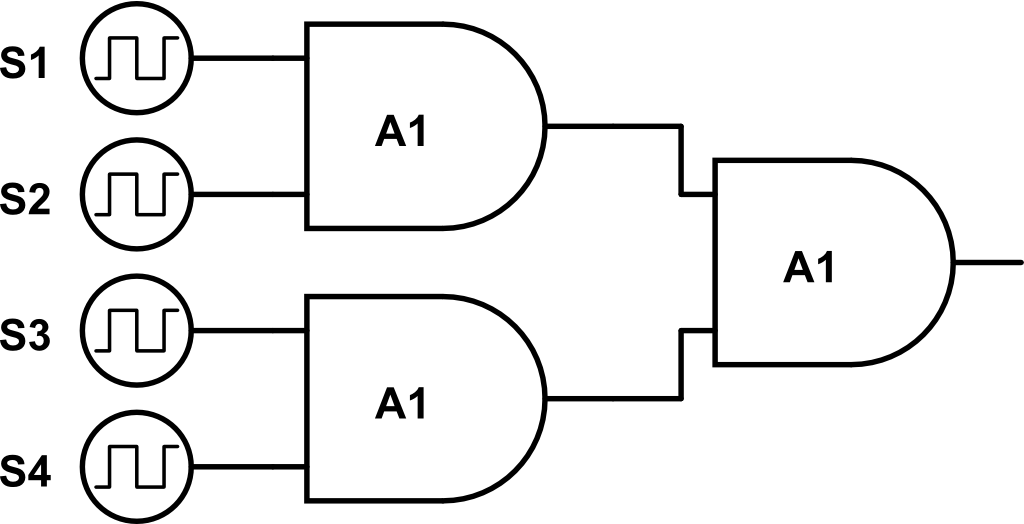
\includegraphics[width=8cm]{../../examples/siggen.png} %TODO: SIGGEN Diagram
 \caption{Circuit diagram of two Signal Generators conencted to a 2-input AND gate}
 \label{fig:example-siggen}
\end{figure}

\pagebreak

\section{EBNF}
\lstinputlisting[caption=EBNF]{../../docs/ebnf.txt} %TODO: define EBNF language

\pagebreak

\section{User Guide}

\pagebreak

\section{File Listing}

\pagebreak
\section{Gantt Chart}
\begin{figure}[h]
 \centering
  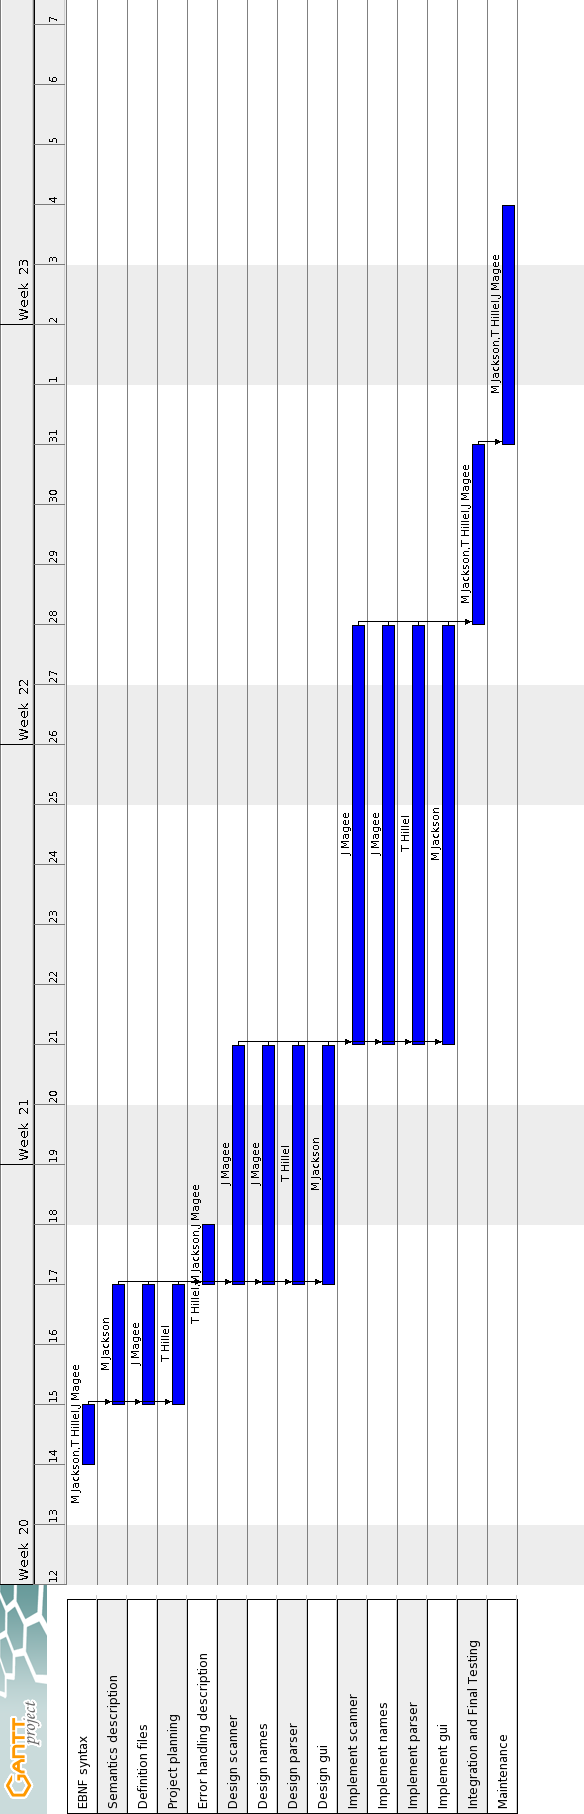
\includegraphics[height=19cm]{Gantt-Chart.png}
 \caption{Gantt chart showing key events in development cycle}
 \label{fig:ganttchart}
\end{figure}
\pagebreak

\section{Class Diagram}
\begin{figure}[h]
 \centering
  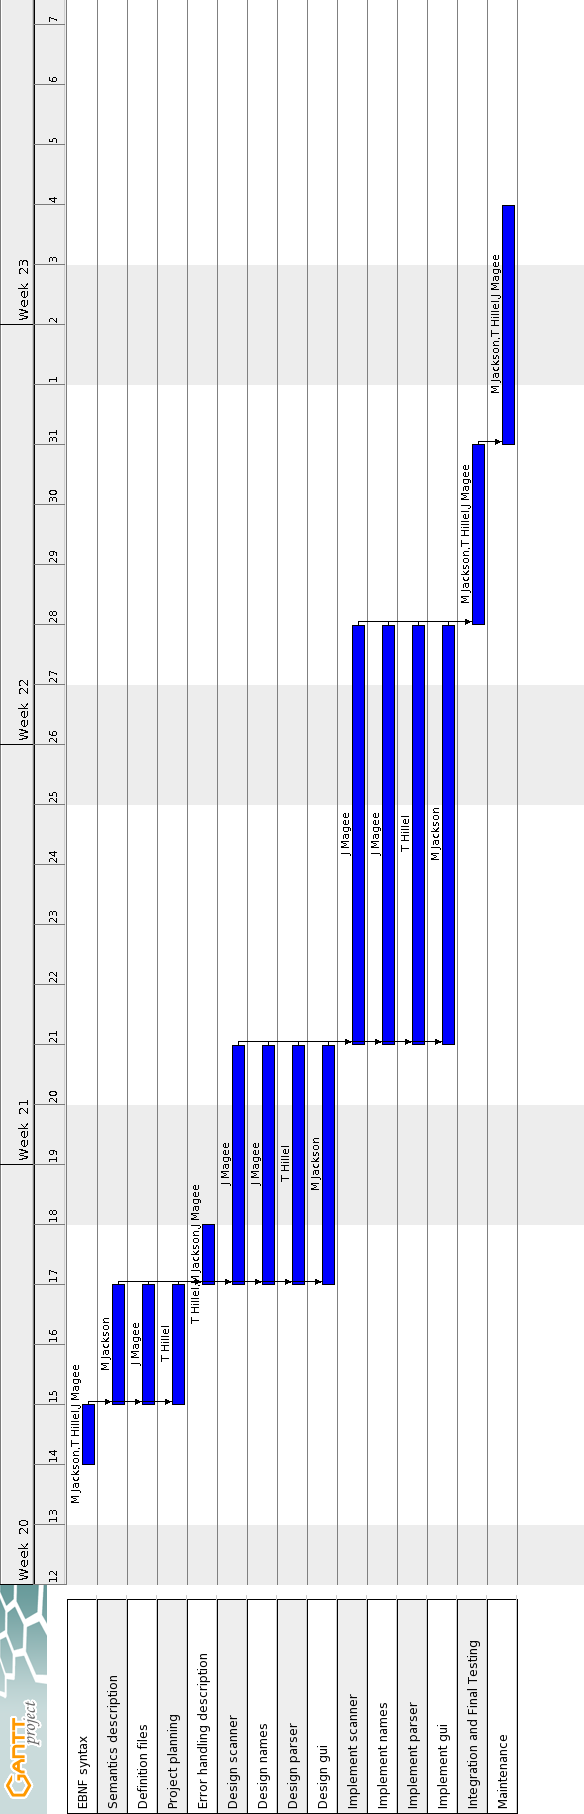
\includegraphics[height=19cm]{Gantt-Chart.png} %TODO: class diagram of logic simulator
 \caption{Class diagram of logic simulator}
 \label{fig:classdiagram}
\end{figure}


\clearpage
\end{document}

